\addcontentsline{toc}{chapter}{Tabella costrutti modello E-R} 

\setlength{\fboxsep}{6pt}
\setlength{\fboxrule}{0pt}
\small
\begin{center}
	\def\arraystretch{1.2}
	\begin{tabular}{ |@{} m{3cm} @{}| m{13cm} | } 
		\hline
		\textbf{Immagine} & \textbf{Descrizione} \\
		\hline
		\multicolumn{2}{|c|}{\textbf{Entità}} \\
		\hline
		\framebox{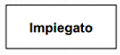
\includegraphics{images/70.PNG}} & \makecell[l]{\parbox{13cm}{\vspace{0.2cm}Classe di oggetti esistenti, presenti nella realtà: persone, cose, città, conti correnti... Ad ogni elemento sono associate proprietà comuni.\\\\\textbf{Occorrenze}: elemento appartenente alla classe\\\textbf{Nomi}: singolari e significativi}}\\
		\hline
		\multicolumn{2}{|c|}{\textbf{Associazione}} \\
		\hline
		\framebox{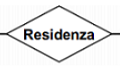
\includegraphics{images/71.PNG}} & \makecell[l]{\parbox{13cm}{\vspace{0.2cm}Legame fra due o più entità. Non ho frecce: non si ha un verso.\\\\\textbf{Occorrenze}: insieme di tuple, di occorrenze di entità.\\\textbf{Nomi}: singolari, significativi, possibilmente senza verbi (no verso).}} \\
		\hline
		\multicolumn{2}{|c|}{\textbf{Attributo}} \\
		\hline
		\framebox{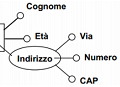
\includegraphics{images/72.PNG}} & \makecell[l]{\parbox{13cm}{\vspace{0.2cm}Proprietà elementari tipiche di un'entità o di un'associazione. Ogni attributo presenta un certo dominio ed è per forza associato ad occorrenze di entità e di associazione.\\\\\textbf{Raggruppamenti}: gli attributi possono essere raffigurati in gruppi (per esempio le informazioni riguardanti un indirizzo).}}\\
		\hline
		\multicolumn{2}{|c|}{\textbf{Cardinalità}} \\
		\hline
		\framebox{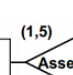
\includegraphics{images/73.PNG}} & \makecell[l]{\parbox{13cm}{\vspace{0.2cm}Coppia di valori che specifica il numero minimo e massimo di occorrenze della relazione a cui può partecipare una occorrenza di entità. Banalmente, indico quante coppie posso stabilire in un'associazione. Presente sia in associazioni che in attributi!\\\\\textbf{Simbologia}: 0 (associazione opzionale) e 1 (associazione obbligatoria) per la cardinalità minima; 1 e N (numero formalmente illimitato di associazioni) per cardinalità massima.}}\\
		\hline
		\multicolumn{2}{|c|}{\textbf{Generalizzazione}} \\
		\hline
		\framebox{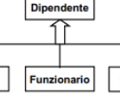
\includegraphics{images/74.PNG}} & \makecell[l]{\parbox{13cm}{\vspace{0.2cm}Costrutto gerarchico che viene perso col passaggio al modello logico. Mi permette di stabilire delle sottoclassi di entità. Presentano degli attributi specifici che li differenziano dalle altre sottoclassi!\\\\\textbf{Tipi}: la generalizzazione è \underline{totale} (freccia piena, genitore occorrenza di almeno uno dei figli), o \underline{parziale} (freccia vuota, genitore non è per forza occorrenza di uno dei figli). La generalizzazione si dice anche \underline{esclusiva} (genitore è occorrenza di al più una delle entità figlie) o \underline{sovrapposta} (genitore occorrenza di più di una delle entità figlio).\\\textbf{Alberi}: posso stabilire degli alberi di gerarchia parallela in cui distinguere generalizzazione totale da quella parziale.}}\\
		\hline
	\end{tabular}
\end{center}